%________________________________________________________________________________________________
\documentclass{beamer}
%________________________________________________________________________________________________
\usepackage[french]{babel} 
\usepackage[utf8]{inputenc} 
\usepackage[T1]{fontenc} 
\usepackage{graphicx}
\usepackage[utf8]{inputenc}
\usepackage{fancyhdr}
\usepackage{geometry}
\usepackage{tabularx,tabulary}
\usepackage{movie15}
%________________________________________________________________________________________________
\title{3I013 Soutenance 6 Mai 2019}
\author{Nicolas CASTANET\\ Maël FRANCESCHETTI\\Daoud KADOCH\\Fabien MANSON\\}
%________________________________________________________________________________________________
%ce theme est le plus clean de Beamer le truc a ne pas utiliser c'est 'Warsaw'
\usetheme{default}
%suppression de la barre de navigation inutile
\setbeamertemplate{navigation symbols}{}
\setbeamertemplate{frametitle}[default][center]

%\logo{
\includegraphics[height=0.5cm]{logo_sorbonne.png}}

%________________________________________________________________________________________________
\addtobeamertemplate{footline}{
	\begin{flushright}
	\vbox{\insertframenumber/\inserttotalframenumber}
	\end{flushright}}

%________________________________________________________________________________________________
\begin{document}


	\begin{frame}
		\begin{center}
		\date{}
		\maketitle
		\end{center}
	\end{frame}
	
%________________________________________________________________________________________________	

	
	%________________________________________________________________________________________________
	
	\begin{frame}
		\section{La Demande du Client}
		\begin{center}
		\frametitle{La Demande du Client}
		\begin{itemize}
		    \item Le client souhaite effectuer des rondes avec un drone Bebop 2\\
		    \item Le drone doit voler de manière autonome en suivant un plan de vol prédéfini \\
		    \item Le retour vidéo du drone doit être redirigé à un iPod touch qui sera placé dans un masque FPV pour permettre à l'utilisateur de voir comme s'il était à la place du drone\\
		\end{itemize}
		   
		\end{center}
	\end{frame}
%________________________________________________________________________________________________	
	\begin{frame}
		\section{Scénario d'Utilisation}
		\begin{center}
		\Large{
			\color{blue}
			
			Scénario d'utilisation
		}
		\end{center}
	\end{frame}
	
%________________________________________________________________________________________________	



%________________________________________________________________________________________________	


	\begin{frame}
		\section{Architecture Matérielle}
		\begin{center}
		\frametitle{Architecture Matérielle}

       %0.6
        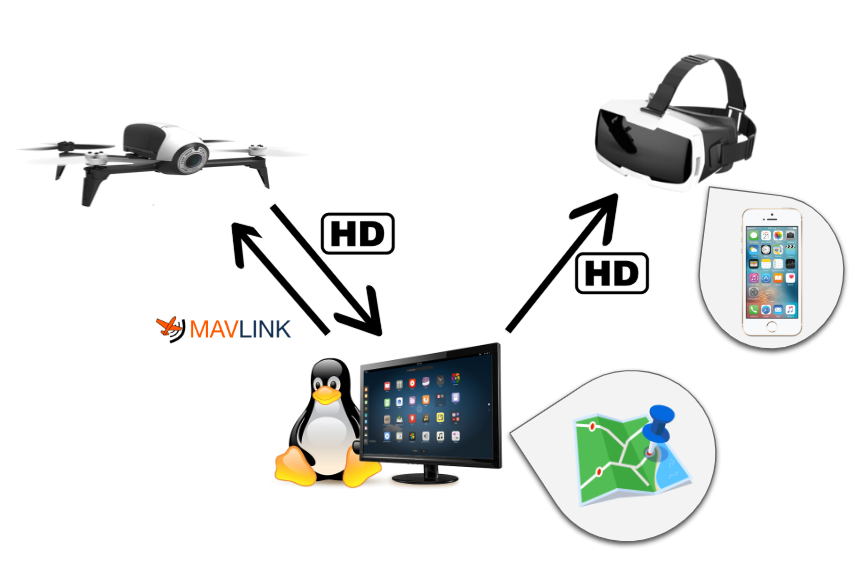
\includegraphics[scale=0.6]{archi_materielle.png}
		\end{center}
	\end{frame}
	
%________________________________________________________________________________________________	


	\begin{frame}
	\section{Architecture Logicielle}
		\begin{center}
		\frametitle{Architecture Logicielle : interface utilisateur}

       	%0.24
        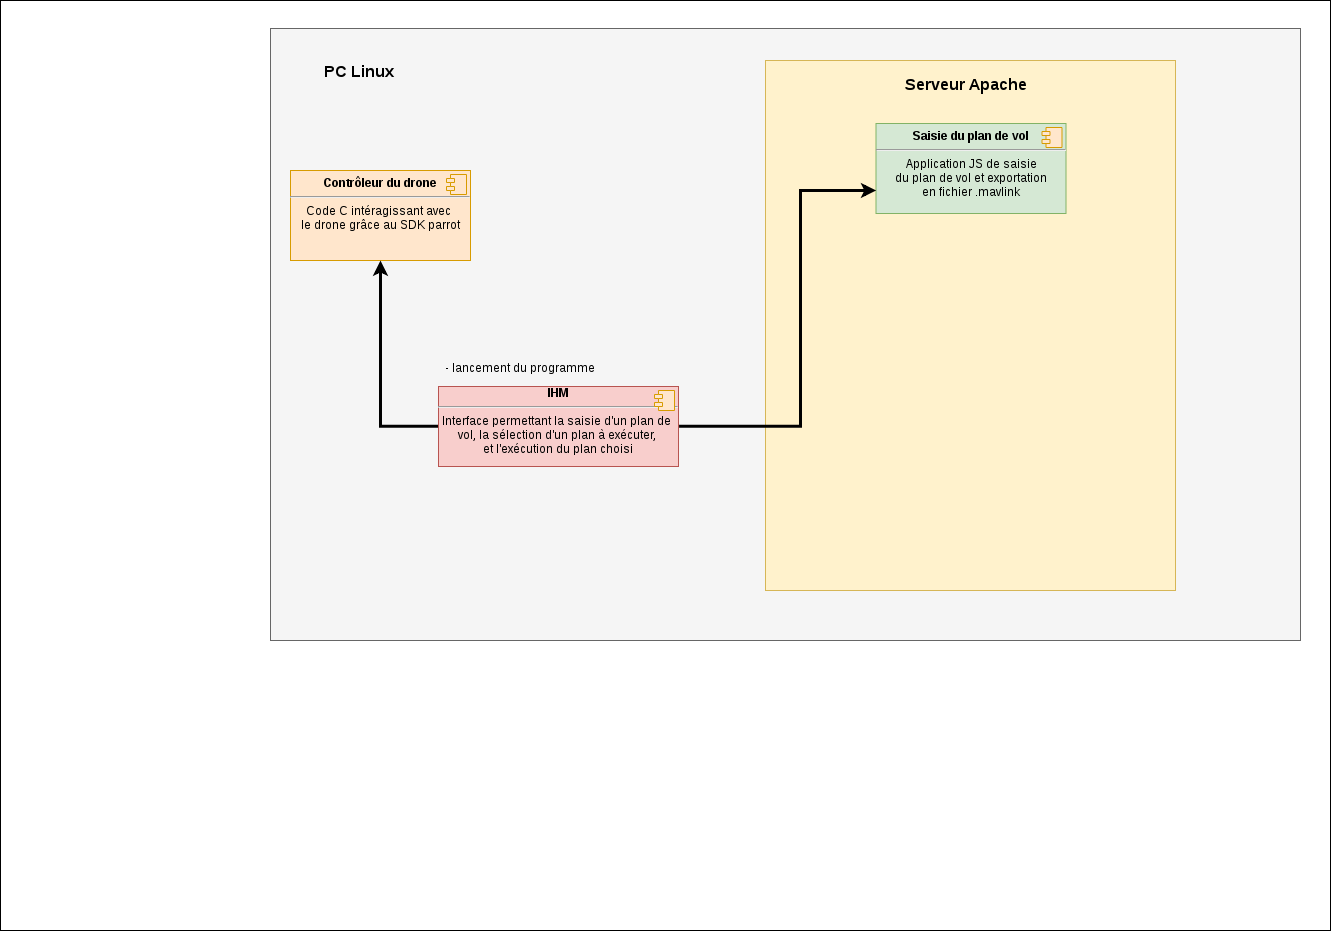
\includegraphics[scale=0.24]{01_archi_logicielle_IHM.png}
		\end{center}
	\end{frame}
	
%________________________________________________________________________________________________


	\begin{frame}
		
		\begin{center}
		\frametitle{Architecture Logicielle : controle du drone}

       
        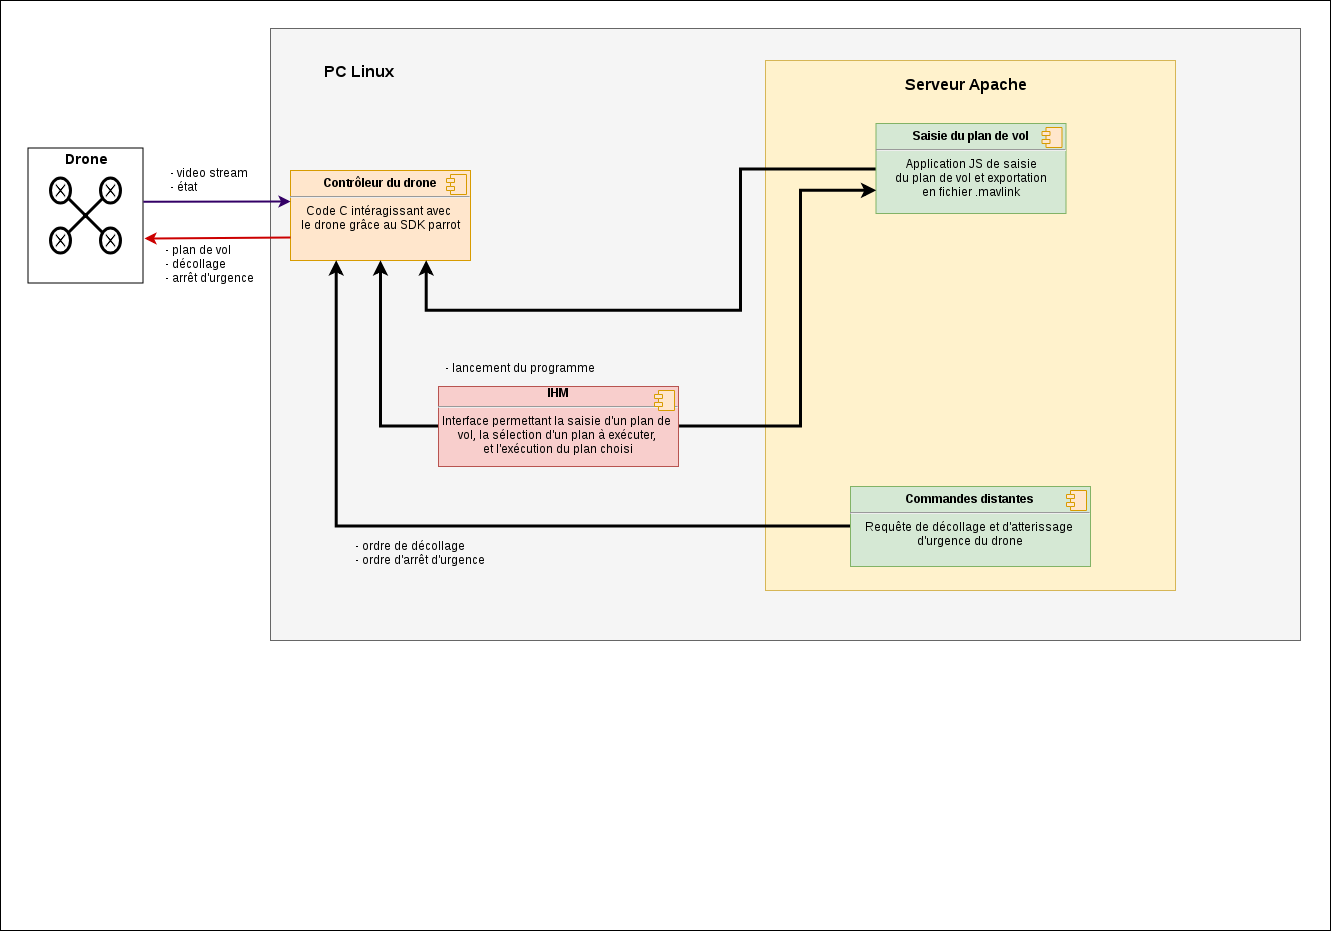
\includegraphics[scale=0.24]{02_archi_logicielle_controle_drone.png}
		\end{center}
	\end{frame}
	
	%________________________________________________________________________________________________

	\begin{frame}
		\begin{center}
		\frametitle{Architecture Logicielle : contrôle avec l'iPod}

       
        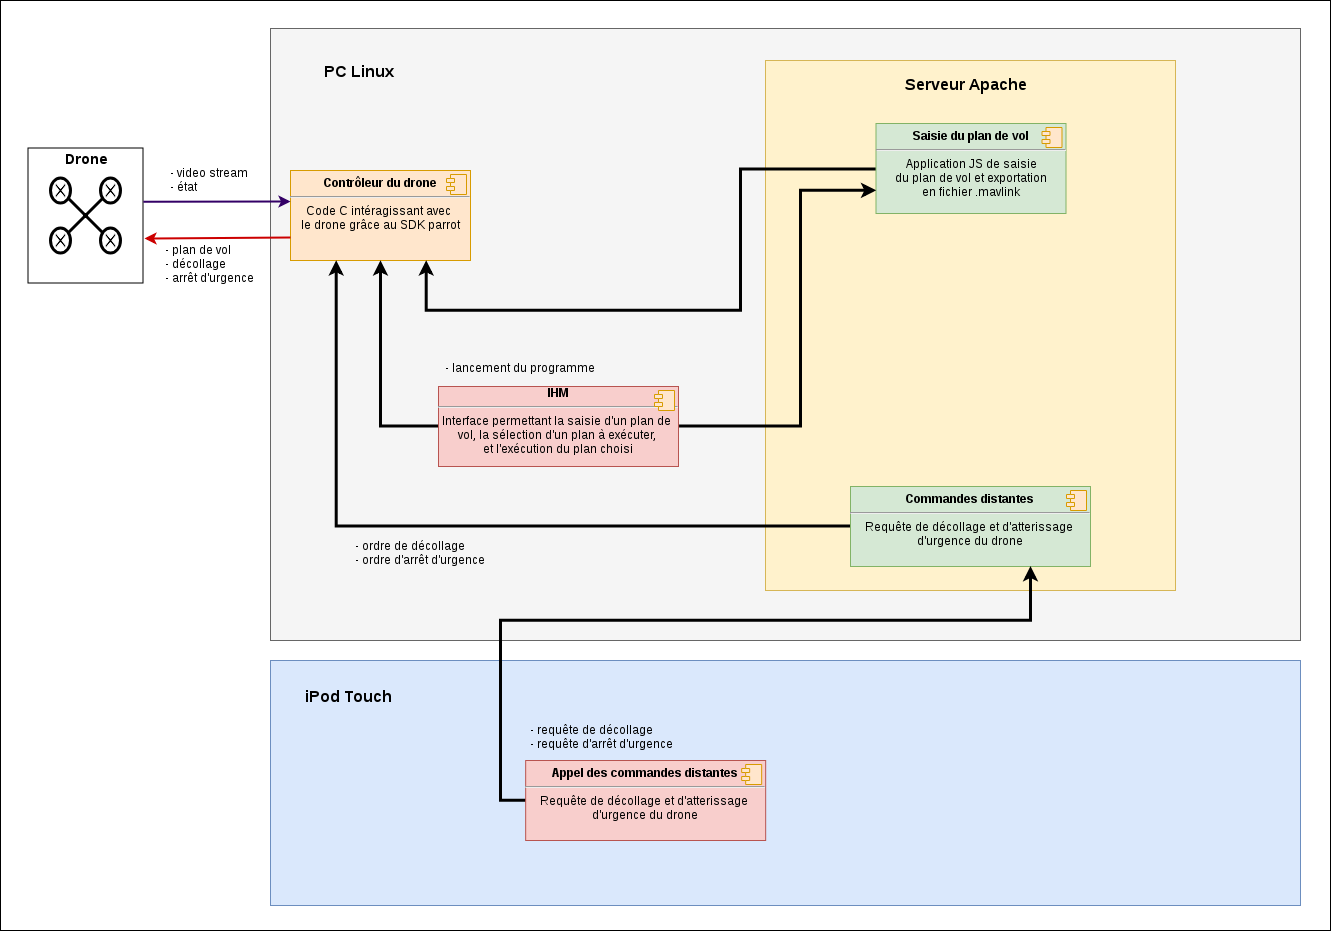
\includegraphics[scale=0.24]{03_archi_logicielle_iPod.png}
		\end{center}
	\end{frame}


%________________________________________________________________________________________________

	\begin{frame}
		\begin{center}
		\frametitle{Architecture Logicielle : retour vidéo sur l'iPod}

       
        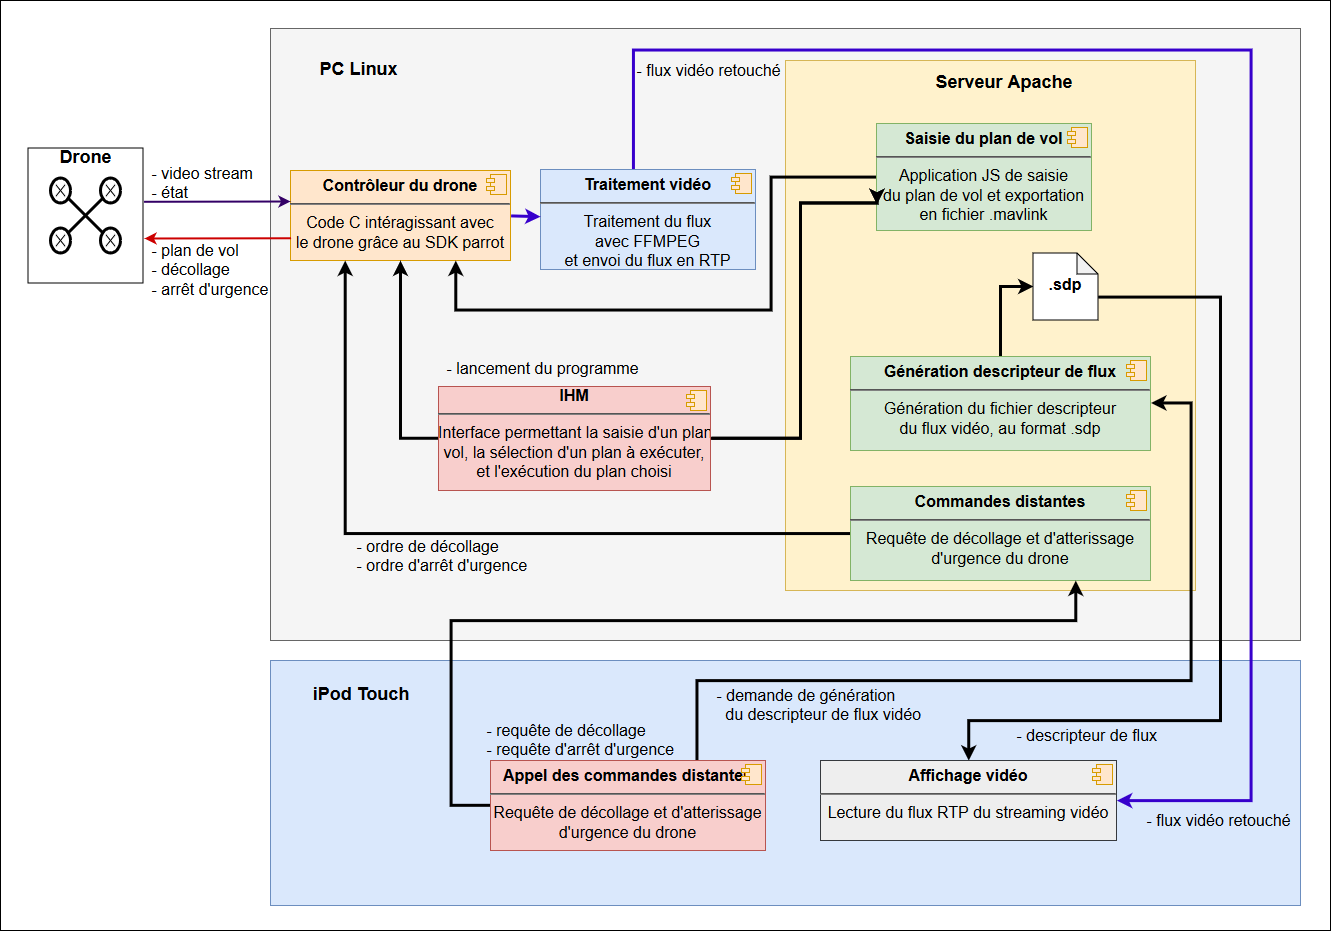
\includegraphics[scale=0.24]{04_archi_logicielle_complete.png}
		\end{center}
	\end{frame}
	
%________________________________________________________________________________________________
	
	
	\begin{frame}
		\section{Test Effectués}
		\begin{center}
		\frametitle{Tests effectués}
           	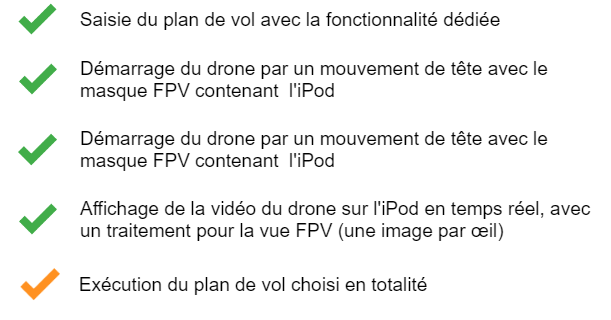
\includegraphics[scale=0.5]{tests.png}
		\end{center}
	\end{frame}

	
%________________________________________________________________________________________________	
	
	\begin{frame}
	\section{Déploiement}
		\begin{center}
		\frametitle{Déploiement}
		\begin{itemize}
	    \item	L'archive contient un script Makefile permettant d'extraire au bon endroit les différents composants de l'application.\\
	    \item	Les outils requis tels que GTK+ 3.0, un serveur Lamp et FFMPEG devront être installés par l'utilisateur au préalable.\\
	    \item	Le serveur devra être paramétré pour donner accès au répertoire "public".\\
		\end{itemize}
		\end{center}
	\end{frame}
	
%________________________________________________________________________________________________	
	
	\begin{frame}
		\begin{center}
		\frametitle{Déploiement : action du Makefile}
		%mettre schéma déploiement
        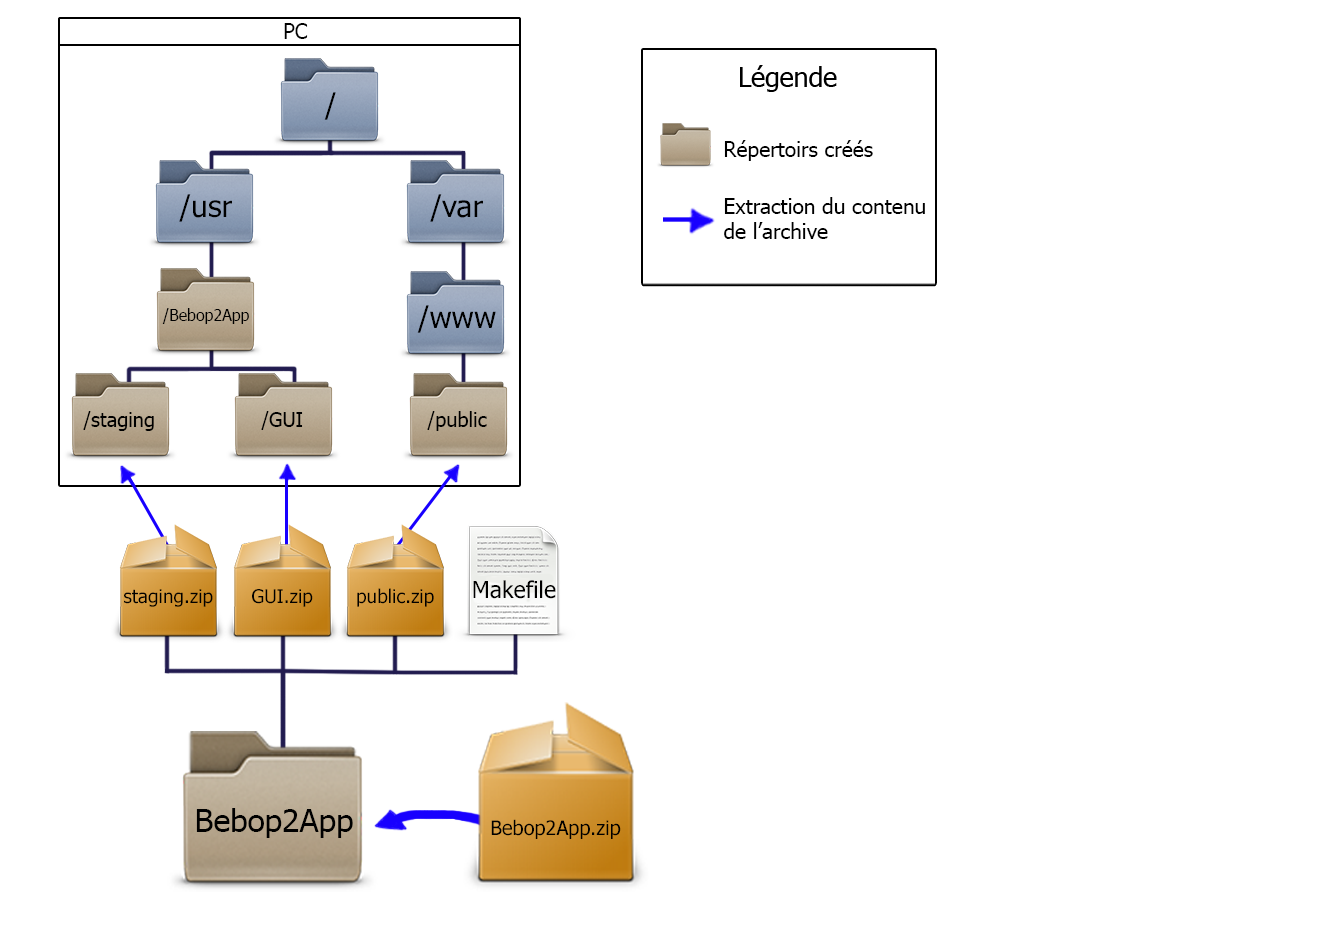
\includegraphics[scale=0.3]{schéma_déploiement_01.png}
		\end{center}
	\end{frame}
	
%________________________________________________________________________________________________	
	
	\begin{frame}
		\begin{center}
		\frametitle{Déploiement : contenu de l'archive}
        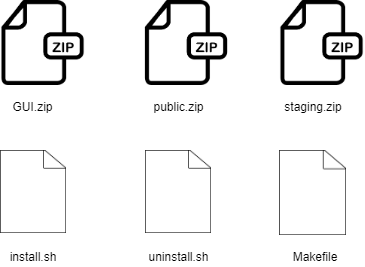
\includegraphics[scale=0.55]{contenu_archive.png}
		\end{center}
	\end{frame}
	
%________________________________________________________________________________________________	
	
	\begin{frame}
		\begin{center}
		\frametitle{Déploiement : make install}
        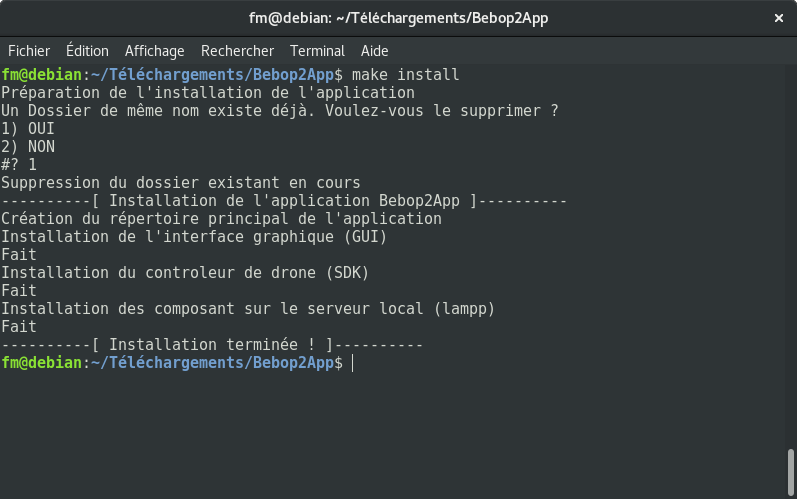
\includegraphics[scale=0.4]{make_install.png}
		\end{center}
	\end{frame}


    \begin{frame}
		\begin{center}
		\frametitle{Déploiement : make uninstall}
        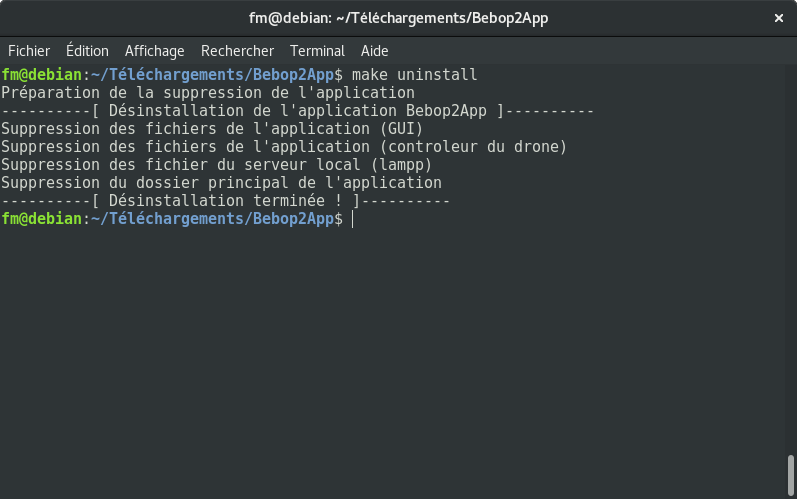
\includegraphics[scale=0.4]{make_uninstall.png}
		\end{center}
	\end{frame}
%________________________________________________________________________________________________	
	% Déploiement : résultat côté controle du drone et IHM


%________________________________________________________________________________________________	
	% Déploiement : résultat côté serveur

%________________________________________________________________________________________________	
	
	\begin{frame}
	\section{Problèmes rencontrés}
		\begin{center}
		\frametitle{Problèmes rencontrés}
        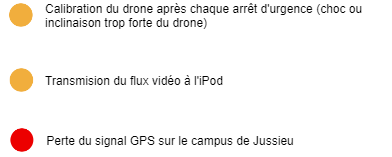
\includegraphics[scale=0.75]{problemes.png}
		\end{center}
	\end{frame}

%________________________________________________________________________________________________	
	
	\begin{frame}
		\section{Répartition du travail}
		\begin{center}
		\frametitle{Diagramme de Gantt}
        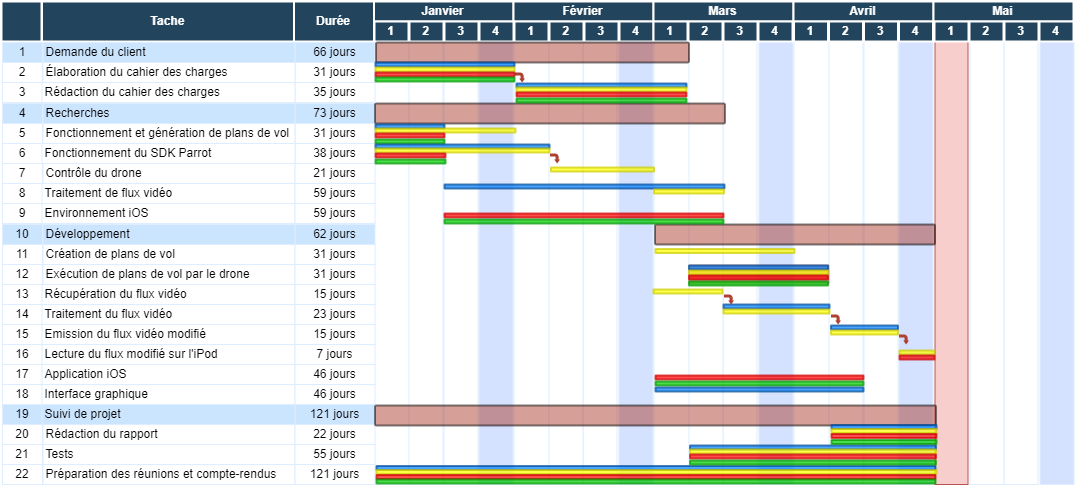
\includegraphics[scale=0.28]{gantt.png}
		\end{center}
	\end{frame}

%________________________________________________________________________________________________	
	
	\begin{frame}
		\begin{center}
		\frametitle{Répartition des tâches}
        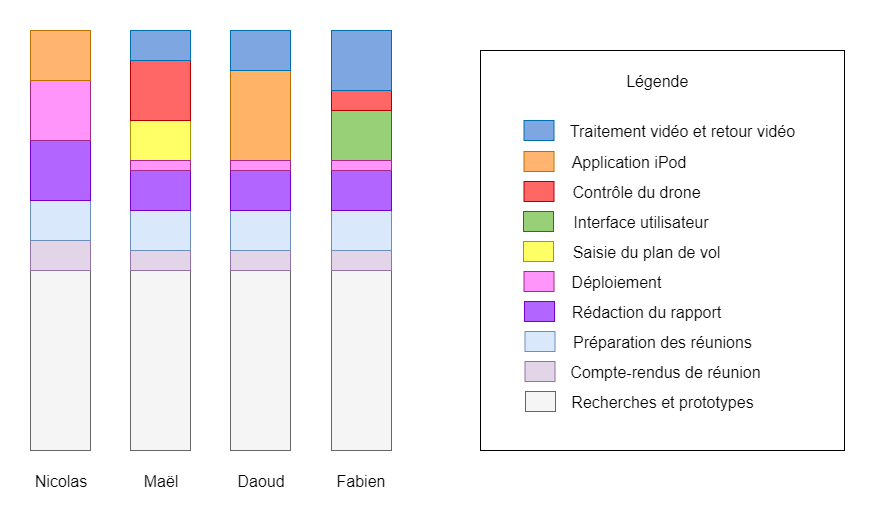
\includegraphics[scale=0.3]{repartition_taches.png}
		\end{center}
	\end{frame}

%________________________________________________________________________________________________	
	
	\begin{frame}
	    \section{Conclusion}
		\begin{center}
		\frametitle{Conclusion}
		\includegraphics[scale=0.05]{drone.JPG}
		\end{center}
	\end{frame}



%________________________________________________________________________________________________	
	
\end{document}
